\chapter{月地返回轨道设计}
\section{月地转移轨道设计}
\subsection{双二体假设下中止轨道计算模型}
设$t_A$时刻进行中止机动,中止点$A$在月心惯性坐标系下的坐标为$r_A^L=[x_A^L\quad y_A^L\quad z_A^L]$,给定出口点经度$\lambda_C$和纬度$\phi_C$,则出口点在月心惯性坐标系下的坐标为

对于跳跃式再入的航天器,初始再入点是冉人轨道的初始点,其位置、速度、速度角将决定再入飞行特性。初始再入点又是月地转移轨道的目标点,受到月地转移轨道的约束。影响初始再入点参数的主要因素有返回时刻、再入角的大小和再入轨道倾角的要求、升轨或降轨到达地球。


\subsection{瞄准参数分析}
\subsubsection{再入角}
再入角只有在飞船到达大气边界才有意义,再入角满足如下的计算方程
\begin{equation}
	\tan \gamma_\mathrm{e}=\frac{1}{R_\mathrm{P}\sqrt{1+e}}\sqrt{-{R_\mathrm{P}}^2(1+e)+2R_\mathrm{e}R_\mathrm{P}-{R_e}^2(1-e)}
\end{equation}
其中,$R_\mathrm{P}$为近地点地心距,$R_\mathrm{e}$为再入点EI的地心距,$e$为地心转移轨道的倾角。
如果$e=1$,则近似有
\begin{equation}
	R_{\mathrm P}=R_{\mathrm{e}}\cos^2\gamma_{\mathrm{e}}
\end{equation}
\subsubsection{再入点经纬度}
再入点处的纬度由月球的赤纬、方向角和再入角决定,与月球的返回时刻相关。再入点的经度受地球自转影响,为短周期项,是返回时间的函数。因此,通过搜索返回时刻与返回时间能够分别满足要求。
\subsubsection{方向角}
方位角和倾角都可以描述再入飞行方向,但是倾角不能确定唯一的飞行方向,因此这里选择方位角描述。不考虑再入过程的横向机动,给定着陆点$F$经纬度$(\theta_{\mathrm f},\phi_{\mathrm f})$和再入点经纬度$(\theta_{\mathrm e},\phi_{\mathrm e})$,根据球面三角公式可以求出瞄准着陆点的标称再入速度方位角,作为月球转移轨道的瞄准参数。

由于防热的原因,设计者希望以较小的大气相对速度再入,而逆行轨道的大气相对速度比顺行轨道更大,所以要求方位角范围在$0\degree\sim 180\degree$之间。

\section{双二体模型下的返回轨道初步设计方法}
在月地转移过程中,飞行器受到地球和月球的引力场作用,地球、月球与飞行器构成限制性三体问题,一般情况下无解析解。

双二体模型是对限制性三体模型的近似,可以分别计算地心段和月心段轨道的解析解,然后将两段轨道拼接为一个整体,也即圆锥曲线拼接法。该方法是
种无需轨道积分的纯代数计算方法,具有收敛速度快的优点,适用于需要大规模计算的参数特性分析,或者作为高精度计算的初值估计。

本节针对月球返回问题建立适应于此问题的新的数学模型。在新的数学模型中,选择物理意乂明确的轨道参数代替出口点经纬度来作为设计变量,可以避免设计参数物理意义不明确的缺点。

\subsection{用到的坐标系}

\begin{enumerate}[label=\arabic*)]
	\item 地心白道系$O_E-XYZ$

		  原点为地心$ O_E $,$ xy $平面为某瞬时$ t_0 $时刻(航天器到达出口点时刻)的白道面, $ x $轴为该时刻由月心指向地心的方向,$ z $轴垂直$ t_0 $时刻的白道面,方向与该时刻月球绕地球公转动量矩方向一致
	\item 月心白道系$O_M-XYZ$

			坐标原点平移,方向与地心白道系$O_E-XYZ$一致。
	\item 月心J2000坐标系

			原点在月心$ O_M $,三轴指向与地心惯性系一致。在此坐标系中与月心白道系转换方便,故用于定义初始月球轨道(LLO轨道根数)
	\item 地心惯性系(ECI)
	\item 地固系(ECF)
\end{enumerate}
\subsection{优化参数(设计变量)选择}
传统的地月空间圆锥曲线拼接方法均采用影响球出口点(或入口点)经度纬度$ \lambda_B,\phi_B $作为设计变量,采用这两个参数可以实现地心段和月心段轨道的拼接计算但作为设计变量却存在不足:1)物理意义不如轨道根数明确,获得它们的分布特性需要通过大量仿真计算;2)需要利用这两个参数结合其它设计变量去推导出地心段和月心段两部分轨道参数,这些轨道参数中有很多本来可以作为输入条件给出的。通过出口点经纬度导出后,在设计模型中有些输入参数却只能作为等式约束存在,增加了额外的等式约束。

{\color{red}参考,}将初始的LLO轨道参数作为模型的输入参数,选择设计变量为:
\begin{enumerate}[label=\arabic*)]
	\item 航天器到达出口点时刻$t_B$
	\item 月心白道系下的出口点纬度幅角$u$
	\item 月心白道系下出口点速度大小$v_{si}$
	\item 加速点A处的速度倾角$\Theta_A$
	      % 在不考虑异面变轨,认为加速脉冲方向沿LO速度方向施加,速度倾角$\Theta_A=0\degree$
\end{enumerate}

\subsection{返回轨道设计动力学模型}
考虑将月球停泊轨道倾角和升交点赤经作为输入条件,同时采用新的具有明显物理意义的设计变量,建立新的返回轨道数学模型

在地心位置矢量$\bm{r}$可表示为
\begin{equation}
	\bm{r}=\bm{r}_M+\bm{r}_{si}
\end{equation}
其中,$\bm{r}_{si}$为B点的月心位置矢量,$\bm{r}_M$为月球的地心位置矢量

出口点速度矢量$v$在地心白道系中矢量表达式为
\begin{equation}
	\bm{v}=\bm{v}_\mathrm{m}+\bm{v}_\mathrm{si}
\end{equation}
其中$ \bm{v}_\mathrm{si} $为出口点速度在月心白道系中矢量,$ \bm{v}_\mathrm{m} $为是月球速度在地心白道系中矢量。

\begin{figure}[htb]
	\centering
	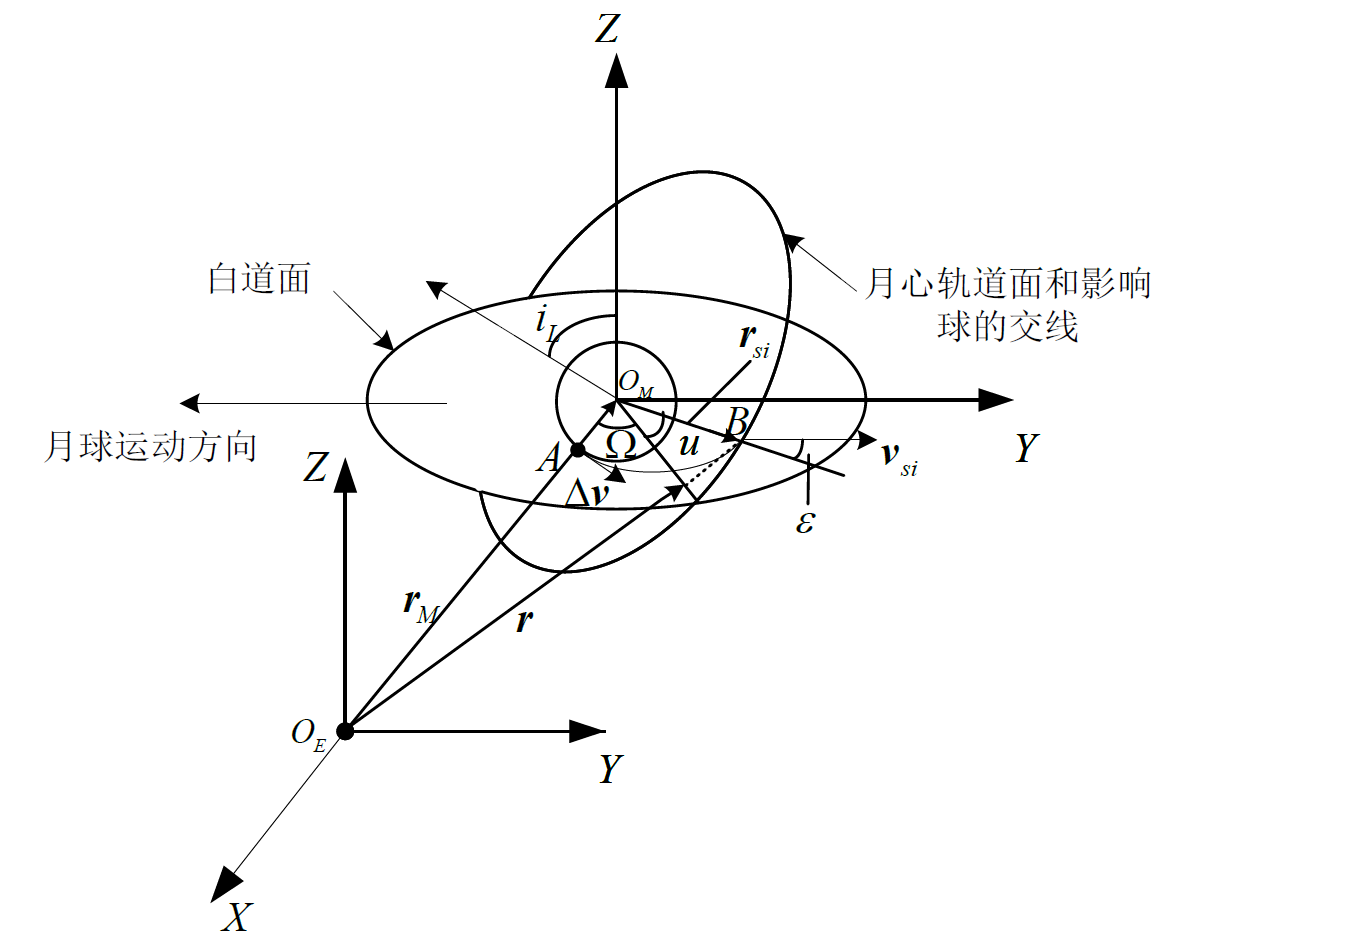
\includegraphics[scale=0.4]{double_two_body_para.png}
	\caption{双二体轨道参数示意图}
	\label{fig:double_two_body_para}
\end{figure}

月心白道系下的出口点位置矢量$\bm{r}_{si}$可以表示为
\begin{equation}
	\bm{r}_{si}^{\mathrm{EMP}}=R_3(-\Omega)R_1(-i)R_3(-u)\left[\begin{array}{c}
			r_{si} \\0\\0
		\end{array}\right]
\end{equation}



进一步考虑月球轨道的非圆性问题,即采用高精度地月运动关系下的圆锥曲线拼接模型进行求解,而不是认为月球是绕地球作匀速圆周运动,这样做在一定程度上能够提髙计算精度。在利用圆锥曲线拼接法求解过程中,所涉及到任何时刻的月球位置和速度均以 JPL DE405星历表为基础得到。$ \bm{v}_\mathrm{m} $可表示为
\begin{equation}
	\bm{v}_\mathrm{m}^{\mathrm{EMP}}=M_{\mathrm{ECI}}^{\mathrm{EMP}}\bm{v}_\mathrm{m}^{\mathrm{ECI}}
\end{equation}
其中,$ M_{\mathrm{ECI}}^{\mathrm{EMP}} $为当前时刻地心惯性系到地心白道系的旋转矩阵。
% 此处的表述选择优化,增加上标EMP,无标记仅代表矢量

假设脉冲$ \Delta v $在LLO面内时,即不考虑异面变轨,$ \bm{v}_\mathrm{si}  $也在月心轨道面内,可以表达为
\begin{equation}
	\begin{aligned}
		\boldsymbol{v}_{\mathrm{si}}^{\mathrm{EMP}}= & R_{3}(-\Omega) R_{1}(-i) R_{3}(-u)  \left[\begin{array}{c}
				v_{s i} \cos \varepsilon \\
				0                        \\
				0
			\end{array}\right]                      \\
		{}                            & +R_{3}(-\Omega) R_{1}(-i) R_{3}\left(-u-90^{\circ}\right)\left[\begin{array}{c}
				v_{s i} \sin \varepsilon \\
				0                        \\
				0
			\end{array}\right]
	\end{aligned}
\end{equation}
其中,$ \epsilon $为出口点位置矢量和速度矢量夹角,可通过月心轨道能量守恒和角动量守恒得到
\begin{equation}\sin \varepsilon=\frac{r_{A}}{r_{s i}} \sqrt{1+\frac{2 \mu_{M}}{r_{A} v_{s i}^{2}}\left(1-\frac{r_{A}}{r_{s i}}\right)} \cos \Theta_{A}\end{equation}

通过将地心位置矢量和速度矢量在地心惯性系下表达,进一步可以求解其他地心轨道参数,近地距、再入角、再入点经纬度、方位角等。初值问题,Lagrange法等,相关计算公式参考郗,相关函数有基础,整理。

\subsection{约束条件分析}
\begin{enumerate}
	\item 优化变量的范围
	
	$ v_1 \leq v_{si} \geq v_{\max} \to f(\Delta v_{\max})$
	\item 航程约束分析

		经过上述计算,可以得到再入点处的位置和速度矢量(地心J2000),着陆点$ (\lambda_f,\phi_f) $已知,通过地固系转换到地心J2000。其中,需要估计再入段航程所用时间。
		根据位置矢量计算航程角$ \delta_R $,
\end{enumerate}
